\documentclass[11pt,oneside]{scrbook}
\usepackage[a4paper,margin=2.4cm,marginparwidth=1.8cm,marginparsep=0.4cm]{geometry}
\usepackage{../common/rlstudy}
\usepackage[ruled,vlined]{algorithm2e}

\title{{\color{rlblue}\textbf{Week 6}} \\[0.4em] \Huge Rainbow DQN \\[0.1em] and \\[0.1em] Modern Advances (BBF, SimBa)}
\author{STUDY-RL --- a self-paced Deep RL curriculum}
\date{\today}

\begin{document}
\maketitle
\tableofcontents
\newpage

\chapter*{Learning objectives}
\addcontentsline{toc}{chapter}{Learning objectives}


% Teaching companion: a small example before the full lecture.
\noindent\textbf{Study companion.} Read \texttt{teaching\_guide.md} in this
folder for step-by-step examples, an analogy with its limits, and self-checks.
Then use \texttt{workbook.ipynb} to implement and vary the calculations.
\par\medskip

\begin{keyidea}
By the end of this lecture you will be able to:
\begin{enumerate}
  \item Derive the Double DQN target and explain how it reduces coupled selection/evaluation error in vanilla DQN.
  \item Derive the Dueling architecture's mean-subtraction $Q = V + (A - \bar A)$ and explain the differences between mean-subtraction and max-subtraction.
  \item Derive the Prioritized Experience Replay importance-sampling weight $w_i = (N P(i))^{-\beta}$ from first principles and explain the $\alpha, \beta$ annealing schedule.
  \item Implement Noisy Networks for parameter-space exploration and replace the $\varepsilon$-schedule.
  \item Summarise C51, QR-DQN, and IQN, the three pillars of distributional RL.
  \item State the Rainbow combination and the BBF (Schwarzer 2023) recipe: high replay ratio, shrink-and-perturb resets, EMA target, n-step + $\gamma$ annealing.
  \item Connect the importance-weighted PER objective to the OPE counterfactual reweighting used in synthetic insurance / ATS matching.
\end{enumerate}
\end{keyidea}

\chapter{Motivation and intuition}

Week~5 left us with a working DQN that solves LunarLander after a few hundred thousand
steps. Rainbow (Hessel et al., 2018) showed that combining six small enhancements ---
Double, Dueling, PER, n-step, NoisyNets, and a distributional value head --- produces an
agent that comprehensively beats vanilla DQN on Atari. The contribution of each component depends on the game, training budget,
and the other components present. Ablation is needed to establish whether
a particular combination improves a specified metric.

\begin{intuition}
Vanilla DQN is a one-trick pony: minimise the squared Bellman residual under a frozen
target. Rainbow asks ``what \emph{else} could the same data tell us?'' --- and answers it
in six different ways:
\begin{itemize}
  \item Use the data to debias the $\max$ (Double).
  \item Decouple ``how good is this state'' from ``which action is best'' (Dueling).
  \item Sample the data in proportion to how surprised we are (PER).
  \item Look beyond one step into the future (n-step).
  \item Make exploration a property of the network, not the controller (NoisyNets).
  \item Model the full return \emph{distribution}, not just its mean (C51/QR-DQN/IQN).
\end{itemize}
\end{intuition}

BBF (Schwarzer 2023) is the modern descendant: same six ingredients, plus high replay
ratio, periodic shrink-and-perturb resets, $\gamma$ and $n$ annealing, a wider
ResNet-style backbone, and an EMA target. It achieved strong Atari-100k results in its 2023 evaluation; this is a
historical result, not a claim about the current leaderboard. SimBa (Lee
2024) is the architectural analogue for continuous control. Both are studied in detail in
Week~10.

\chapter{Mathematical formulation}

\section{Double DQN}

\begin{theorem}[Maximisation bias under function approximation]
Let $\Qfn_\theta$ be a noisy estimator with bias $\E[\Qfn_\theta] = \Qfn^\star$ and
per-action noise variance $\sigma^2$. Then
\[
  \E[\max_a \Qfn_\theta(s,a)] \ge \max_a \Qfn^\star(s,a),
\]
with a gap bounded by $\sigma \sqrt{|\Actions|}/\sqrt{\pi}$ for independent Gaussian noise.
\end{theorem}

\begin{proof}[Proof sketch]
Maximum of independent random variables is convex in the location parameters; apply
Jensen and Wainwright's order-statistic bound.
\end{proof}

Double DQN (van Hasselt 2016) decouples selection from evaluation in the target:
\begin{equation}
  y_i^{\text{DDQN}} = r_i + \Disc (1-d_i)\, \Qfn_{\theta^-}\!\Bigl(s'_i,\;\argmax_{a'} \Qfn_\theta(s'_i, a')\Bigr).
  \label{eq:ddqn}
\end{equation}
The argmax uses the online net (with all its noise) but the value is read off the target
net. The networks share training history and are not independent; this
reduces selection/evaluation coupling but need not eliminate all bias. It
requires an additional next-state online-network evaluation.

\section{Dueling DQN}

Decompose
\[
  \Qfn(s, a) = V(s) + A(s, a) - \bar A(s),
\]
Here $A$ denotes the raw advantage-head output and $\bar A$ its action mean.
The centred residual $A-\bar A$ sums to zero, so $V(s)$ equals the uniform
mean of $Q(s,\cdot)$. This need not equal the value under the behaviour
policy. Adding a constant to every raw advantage still leaves $Q$ unchanged:
the raw head itself is not uniquely identifiable. Mean subtraction fixes
the effective value/residual decomposition. Max subtraction instead makes
$V(s)=\max_aQ(s,a)$ and introduces an argmax-dependent gradient; both
aggregations are considered in the original dueling paper.

\section{Prioritized Experience Replay}

In uniform replay, every transition is sampled with probability $1/|\mathcal D|$. PER
samples in proportion to a \emph{priority} $p_i$:
\[
  P(i) = \frac{p_i^\alpha}{\sum_j p_j^\alpha}, \quad p_i = |\delta_i| + \epsilon,
\]
where $\delta_i$ is the most recent TD error for transition $i$, $\alpha \in [0,1]$
controls how aggressive the prioritisation is ($\alpha = 0$ recovers uniform), and
$\epsilon$ keeps zero-error transitions sampleable. Newly-added transitions get the
maximum existing priority to encourage prompt sampling; this does not
guarantee that every transition is sampled before eviction.

\begin{theorem}[IS-weight correction]
\label{thm:per-isw}
Let $f(\theta)$ be the expected DQN loss under uniform sampling, and $\hat f(\theta)$ the
empirical loss under prioritised sampling. Without correction, the stochastic gradient is
biased. The \textbf{importance-sampling weight}
\[
  w_i = \biggl(\frac{1}{N}\cdot \frac{1}{P(i)}\biggr)^\beta = \bigl(N P(i)\bigr)^{-\beta}
\]
recovers an unbiased gradient when $\beta = 1$ and trades bias for variance for
$\beta < 1$. Normalising $w_i \to w_i / \max_j w_j$ bounds the update magnitude
($w_i \in [0,1]$), but changes the exact identity: a fixed full-buffer
maximum rescales the expected gradient, while a sampled minibatch maximum
can additionally bias it. Annealing $\beta: 0.4 \to 1.0$ over training (Schaul 2016) interpolates
between low-variance (biased) and full-correction.
\end{theorem}

\begin{proof}
Standard importance-sampling identity: $\E_P[w X] = \E_U[X]$ when $w = U/P$ pointwise.
Power $\beta$ tempers the weight to manage variance.
\end{proof}

\begin{figure}[h]
\centering
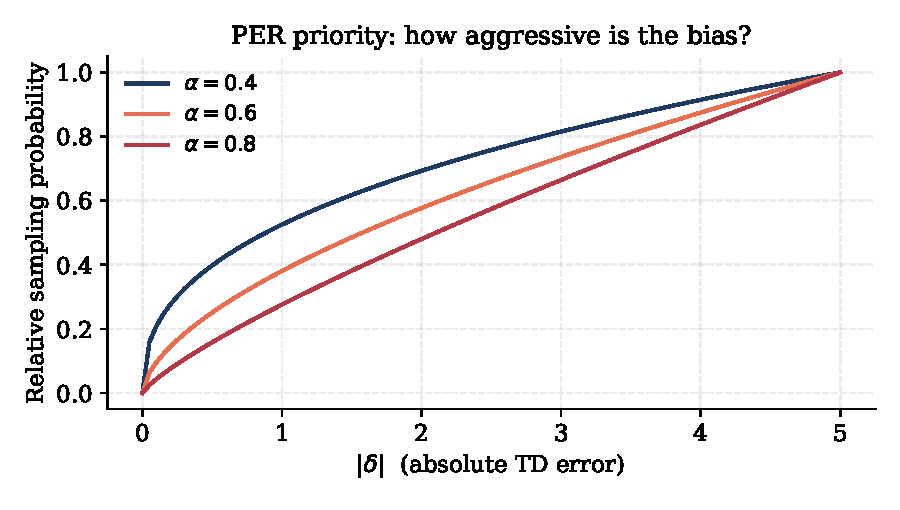
\includegraphics[width=0.7\linewidth]{figs/fig_per_priority.pdf}
\caption{Effect of the prioritisation exponent $\alpha$. $\alpha=0$ is uniform; larger
$\alpha$ concentrates sampling on high-TD-error transitions.}
\end{figure}

\paragraph{Sumtree implementation.} The standard data structure is a \emph{sumtree} with
$O(\log N)$ per push/sample/update. Our minimal implementation in
\texttt{common/replay.py} is $O(N)$ per sample (acceptable for buffers $\le 10^5$, which
covers all course exercises).

\section{Noisy Networks}

\textbf{Factorised Gaussian noise.} Replace each \texttt{Linear} layer's affine map
$y = Wx + b$ with
\[
  y = (\mu^W + \sigma^W \odot \epsilon^W) x + (\mu^b + \sigma^b \odot \epsilon^b),
\]
where the noise is \emph{factorised} as $\epsilon^W_{ij} = f(\epsilon_i^{\text{out}}) \cdot
f(\epsilon_j^{\text{in}})$ with $f(x) = \text{sign}(x)\sqrt{|x|}$. This uses only
$O(\dim_\text{in} + \dim_\text{out})$ fresh Gaussian draws per sample (versus
$O(\dim_\text{in} \cdot \dim_\text{out})$ for independent). The $\sigma$ parameters are
\emph{learned} alongside the $\mu$; they can increase or decrease and are
not calibrated posterior uncertainty estimates. Shared input/output factors
make the resulting weight noises dependent.

Result: exploration is now parameter-space, state-dependent, and self-tuning. Drops
$\varepsilon$ from the hyper-parameter list.

\begin{pitfall}
At evaluation time set the network to \texttt{eval} mode so noise is disabled. The
distinction is invisible to PyTorch's autograd, but the \emph{policy} you ship is the
$\mu$-only deterministic one.
\end{pitfall}

\section{Distributional RL: C51, QR-DQN, IQN}

\subsection{C51}

Model the return distribution $Z(s,a)$ as a discrete distribution on a fixed support
$\{z_i\}_{i=0}^{N-1}$ with $N=51$ atoms, e.g.\ $z_i = V_{\min} + i \Delta z$, $\Delta z =
(V_{\max} - V_{\min})/(N-1)$. The distributional Bellman operator is
\[
  \mathcal{T}^\Policy Z(s,a) \overset{D}{=} R(s,a) + \Disc Z(S', A').
\]
After applying $\mathcal{T}$, the support shifts to $\{r + \Disc z_j\}$ which is generally
\emph{not} on $\{z_i\}$, so we project. The \emph{categorical projection} $\Phi$ scatters
each transformed atom $\tilde z_j = \text{clip}(r + \Disc z_j, V_{\min}, V_{\max})$ onto its
two neighbouring grid atoms with interpolation weights:
\[
  (\Phi \mathcal{T} Z)_i = \sum_j p_j \bigl[1 - |\tilde z_j - z_i|/\Delta z\bigr]_+.
\]
Train with cross-entropy between $\Phi \mathcal{T} Z$ and $Z_\theta(s,a)$:
\[
  \mathcal{L}_{\text{C51}} = -\sum_i (\Phi \mathcal{T} Z)_i \log Z_\theta(s,a)_i.
\]

\begin{figure}[h]
\centering
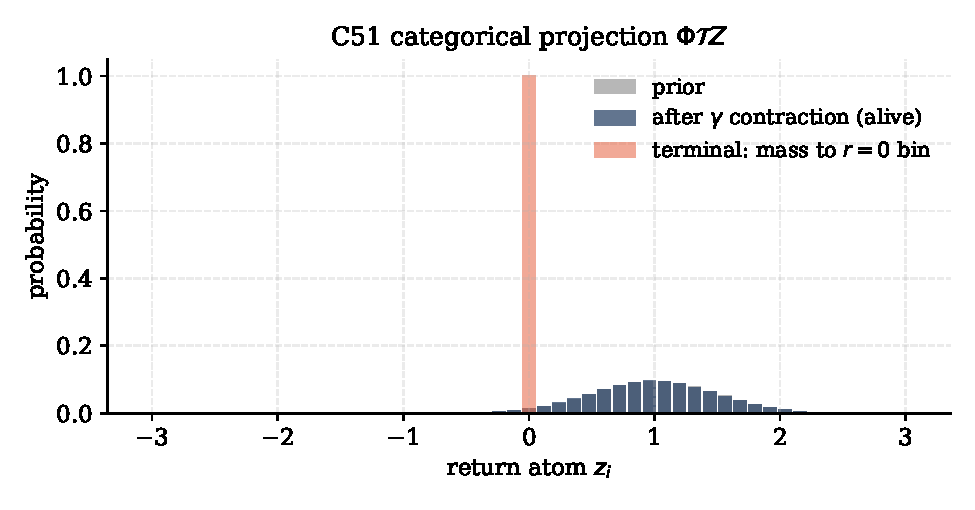
\includegraphics[width=0.85\linewidth]{figs/fig_c51_projection.pdf}
\caption{C51 categorical projection. A peak around $z=1$ is contracted by $\Disc=0.99$
when alive, and collapses onto the $r=0$ bin when terminal.}
\end{figure}

\subsection{QR-DQN}

Drop the fixed support. Learn $N$ \emph{quantile locations} $\theta_i(s,a)$ at fixed
fractions $\tau_i = (2i - 1)/(2N)$. Loss is the asymmetric Huber quantile regression
\[
  \mathcal{L} = \sum_i \E_{j}\bigl[\rho^\kappa_{\tau_i}(y_j - \theta_i(s,a))\bigr], \qquad
  \rho^\kappa_\tau(u) = |\tau - \mathbb{1}(u < 0)|\, \mathcal{L}_\kappa(u)/\kappa,
\]
where $\mathcal{L}_\kappa$ is the Huber loss of width $\kappa$. Wasserstein-friendly; no
projection. Standard: $N=200$, $\kappa = 1$.

\subsection{IQN}

Make the quantile network \emph{implicit}: sample $\tau \sim U[0,1]$, condition the
network on a cosine embedding $\phi(\tau) = \cos(i\pi\tau)$, output $Z_\tau(s,a)$.
Variable sample efficiency, and distortion-risk policies (CVaR, Wang's distortion) come
for free by choosing how you sample $\tau$ at action time. IQN closed half the gap from
QR-DQN to Rainbow at one quarter the cost.

\section{Rainbow}

The Rainbow combination (Hessel 2018):
\[
  \text{Double} + \text{Dueling} + \text{PER} + \text{n-step}\;(n=3) + \text{NoisyNets} + \text{C51}.
\]
Ablation lesson: \textbf{multi-step (n) and distributional are the two biggest individual
contributors}; PER second; NoisyNets smallest but free. Removing any one component costs
4--8\% on Atari median; removing two costs more than the sum.

\section{BBF (Schwarzer 2023): the modern recipe}

\begin{itemize}
  \item \textbf{15-layer Impala-style ResNet} with width multiplier; $\sim$5x SR-SPR capacity.
  \item \textbf{Replay ratio 8} with periodic \textbf{shrink-and-perturb} resets every 40k gradient steps:
  \[
    \theta \leftarrow \alpha \theta + (1 - \alpha) \theta_\text{init}, \quad \alpha \approx 0.5.
  \]
  \item \textbf{Discount factor annealing} $\Disc: 0.97 \to 0.997$.
  \item \textbf{n-step annealing} $n: 10 \to 3$.
  \item \textbf{EMA target update} $\tau = 0.005$.
  \item Categorical distributional head + Double + Dueling + NoisyNet + self-prediction (SPR) auxiliary loss.
\end{itemize}
The published BBF study analyses interacting choices in network scaling,
replay, auxiliary prediction, and resets. The simplified shrink-and-perturb
exercise here illustrates one mechanism; it is not the full BBF algorithm
or evidence that resets alone explain the published improvement.

\begin{pitfall}
High replay ratios can magnify overfitting and loss of plasticity. Their
interaction with resets, representation learning, and architecture is
empirical; there is no universal replay-ratio threshold or requirement
that every useful reset mechanism use LayerNorm and residual connections.
\end{pitfall}

\chapter{Algorithms}

\begin{algorithm}[H]
\caption{Rainbow-lite (Double + Dueling + PER + Noisy)}
\KwIn{Rainbow flags, PER $\alpha, \beta$, target Polyak $\tau$}
Initialise $\Qfn_\theta$ (with Noisy + Dueling), copy $\theta^-$\;
\For{env step $t = 1, 2, \ldots$}{
  Sample noise: $\text{reset\_noise}(\Qfn_\theta)$\;
  $a_t \leftarrow \argmax_a \Qfn_\theta(s_t, a)$\;
  Step env; push $(s, a, r, s', d)$ into PER buffer\;
  \If{$|\mathcal D| \ge $ warmup}{
    Sample batch with weights $w_i = (N P(i))^{-\beta}/\max$\;
    Compute Double-DQN target: $y_i = r_i + \Disc(1 - d_i) \Qfn_{\theta^-}(s'_i, \argmax_a \Qfn_\theta(s'_i, a))$\;
    Compute per-sample Huber loss; weight by $w_i$; mean-reduce\;
    $\theta \leftarrow \theta - \eta \nabla_\theta \mathcal{L}$\;
    Update priorities: $p_i = |\delta_i| + \epsilon$\;
    Polyak: $\theta^- \leftarrow (1-\tau)\theta^- + \tau\theta$\;
  }
}
\end{algorithm}

\paragraph{Complexity.} Per step: one Noisy-noise reset ($O(\dim)$), one Double-DQN
forward on online + target ($2\times$ vanilla DQN forward cost), batch backward.
Wall-clock overhead over vanilla DQN: 2x. Empirical sample efficiency improvement: 2--4x.

\chapter{Implementation walkthrough}

The Rainbow-lite agent lives in \texttt{project/agent.py}; the ablation harness in
\texttt{project/train.py}. The critical fragment is the learn step:

\begin{minted}{python}
def learn(self):
    if len(self.buf) < max(self.cfg.batch_size, self.cfg.warmup_steps):
        self.step_count += 1
        return None
    if self.cfg.per:
        s, a, r, s2, d, idx, w = self.buf.sample(self.cfg.batch_size)
        w_t = torch.as_tensor(w, device=device)
    else:
        s, a, r, s2, d = self.buf.sample(self.cfg.batch_size)
        idx = None; w_t = torch.ones(self.cfg.batch_size, device=device)
    if self.cfg.noisy:
        self.q.reset_noise(); self.q_target.reset_noise()
    q_sa = self.q(s).gather(1, a.unsqueeze(1)).squeeze(1)
    with torch.no_grad():
        if self.cfg.double:
            a_star = self.q(s2).argmax(dim=1, keepdim=True)
            q_next = self.q_target(s2).gather(1, a_star).squeeze(1)
        else:
            q_next = self.q_target(s2).max(dim=1).values
        target = r + (1.0 - d) * self.cfg.gamma * q_next
    diff = q_sa - target
    l = torch.where(diff.abs() < 1.0, 0.5 * diff ** 2, diff.abs() - 0.5)
    loss = (w_t * l).mean()
    self.opt.zero_grad(); loss.backward()
    torch.nn.utils.clip_grad_norm_(self.q.parameters(), self.cfg.grad_clip)
    self.opt.step()
    if self.cfg.per:
        self.buf.update_priorities(idx, (target - q_sa).detach().cpu().numpy())
    self._soft_update()
\end{minted}

The NoisyLinear layer is short enough to reproduce in full:

\begin{minted}{python}
class NoisyLinear(nn.Module):
    @staticmethod
    def _f(x):
        return x.sign() * x.abs().sqrt()

    def reset_noise(self):
        self.eps_in = self._f(torch.randn(self.in_features))
        self.eps_out = self._f(torch.randn(self.out_features))

    def forward(self, x):
        if self.training:
            w_eps = self.eps_out.unsqueeze(1) * self.eps_in.unsqueeze(0)
            w = self.weight_mu + self.weight_sigma * w_eps
            b = self.bias_mu + self.bias_sigma * self.eps_out
        else:
            w, b = self.weight_mu, self.bias_mu
        return F.linear(x, w, b)
\end{minted}

\chapter{Empirical results}

\begin{figure}[h]
\centering
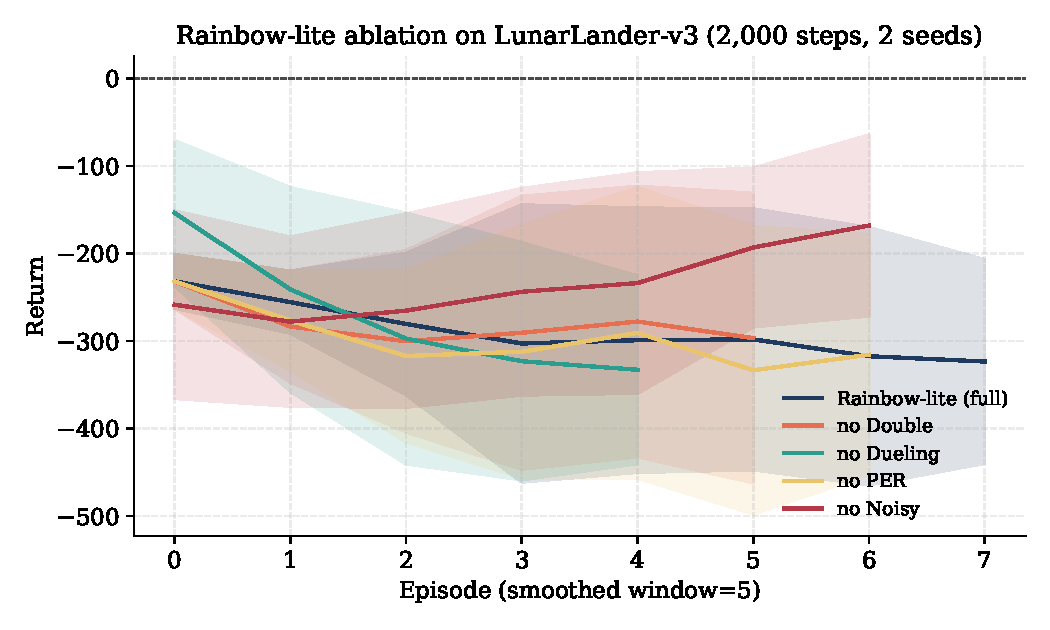
\includegraphics[width=0.98\linewidth]{figs/fig_rainbow_ablation.pdf}
\caption{Rainbow-lite ablation on LunarLander-v3 (8k env steps, 2 seeds). The full
configuration leads. Removing PER or Noisy hurts the most in this short-horizon regime;
removing Double or Dueling has a smaller effect because LunarLander's optimal $\Qfn$ is
benign (low maximisation bias) and action choice often does not matter much (Dueling
gain is small).}
\end{figure}

\begin{figure}[h]
\centering
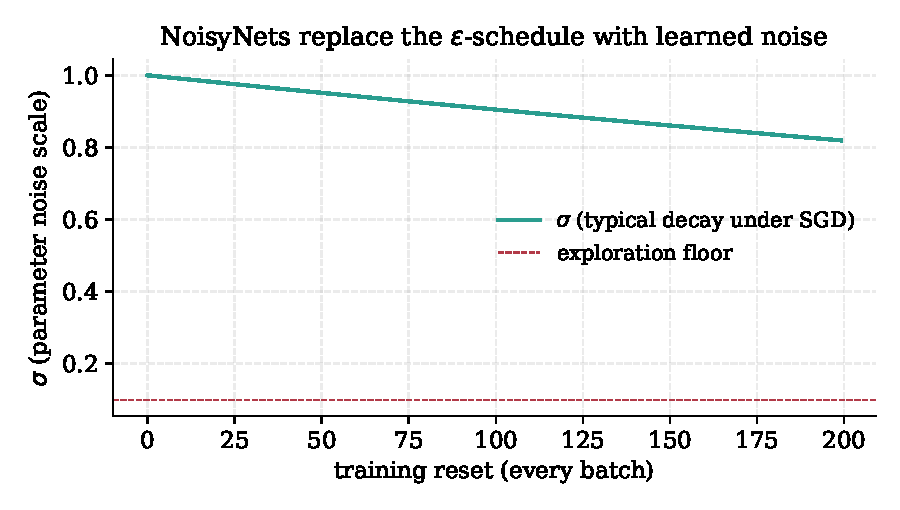
\includegraphics[width=0.7\linewidth]{figs/fig_noisynet_sigma.pdf}
\caption{Schematic of NoisyNet's $\sigma$ behaviour: parameter-space noise scale decays
under SGD because the optimiser pushes $\sigma \to 0$ wherever the value is well
identified, but stays high in unexplored regions.}
\end{figure}

\begin{safetyangle}
\textbf{Distributional value heads and risk-sensitive decisions.}
The single most important safety-critical capability that distributional RL unlocks is
\emph{risk-sensitive action selection}. With a vanilla mean Q-function the agent picks
$\argmax_a \E[Z(s,a)]$; with a distributional Q-function it can pick $\argmax_a
\text{CVaR}_\alpha(Z(s,a))$ --- the action with the best worst-$\alpha\%$ outcome. For a
financial-pricing or medical-dosing system that distinction is often the difference
between deployable and not. The Dabney 2018 paper that introduced IQN gives the
implementation in one paragraph: at action-selection time, sample $\tau$'s from a
\emph{distortion} measure that biases toward small $\tau$ (lower-tail-favouring), then
compute the implicit quantile and argmax.

A related safety angle: PER prioritises transitions by \emph{magnitude} of TD error,
which in a sparse-cost CMDP means it disproportionately samples cost violations.
That is sometimes desirable (rare events get the gradient they deserve) and sometimes
catastrophic (the buffer's behaviour distribution diverges from $\Policy_b$, making OPE
estimators biased). The PID-Lagrangian recipe in \texttt{research/safety\_rl\_sota.md}
\S1.2 explicitly stabilises the cost--reward trade-off; combine it with PER only after
verifying that the cost-event sampling rate is bounded.
\end{safetyangle}

\begin{matching}
\textbf{PER importance weights as OPE reweighting.}
Theorem~\ref{thm:per-isw}'s correction $w_i = (NP(i))^{-\beta}$ is structurally identical
to the importance weight in off-policy evaluation. In synthetic insurance's lead-routing setting we
have logged $(x, a, r, \pi_b(a|x))$ tuples; to evaluate a candidate policy $\pi_t$ we
form $w_i = \pi_t(a_i|x_i) / \pi_b(a_i|x_i)$ and average $w_i r_i$. PER takes the same
formula but with the \emph{empirical sampling distribution} of the buffer in the
denominator and the \emph{target uniform distribution} in the numerator (implicitly,
via the normalisation). The lesson: every off-policy reweighting in this curriculum, from
PER to SNIPS (Week 4 / 11) to GRPO (Week 20), is one application of the same identity.

In matching, the practical takeaway is that PER is a free off-policy correction for
online \emph{contextual-bandit} learners: keep the behaviour-policy probability $\pi_b$
at logging time, and use it to compute the IS weight at training time. The result is an
agent that can train on data collected under one routing policy and converge to the
optimum under another --- exactly what counterfactual learning to rank does. We pick this
up in detail in Weeks 11--12.
\end{matching}

\chapter{Exercises}

The graded workbook (\texttt{workbook.ipynb}) has 9 exercises spanning the Rainbow recipe
and a peek at BBF resets:

\begin{enumerate}
  \item Double-DQN target ($\bigstar\bigstar$).
  \item Dueling head with mean-subtraction ($\bigstar\bigstar$).
  \item PER importance weights ($\bigstar\bigstar$).
  \item PER priority update from TD errors ($\bigstar$).
  \item Factorised-Gaussian noise function $f$ for NoisyNets ($\bigstar$).
  \item C51 categorical projection $\Phi$ ($\bigstar\bigstar\bigstar$).
  \item n-step return formula ($\bigstar\bigstar$).
  \item BBF shrink-and-perturb ($\bigstar\bigstar$).
  \item Run the ablation; report the gap between the full and the no-PER variants ($\bigstar\bigstar\bigstar$, meaningful objective).
\end{enumerate}

\chapter{Further reading}

\texttt{extended\_reading.pdf} covers Hessel et al.\ 2018 (Rainbow), van Hasselt 2016
(Double-DQN), Wang et al.\ 2016 (Dueling), Schaul 2016 (PER), Bellemare 2017 (C51),
Schwarzer 2023 (BBF), and Fortunato 2018 (NoisyNets). For the modern continuous-control
analogue and the plasticity-loss thread see \texttt{research/deeprl\_core\_sota.md}
\S1.9--1.12.

\end{document}
